% !TEX encoding = UTF-8 Unicode
%%%%%%%%%%%%%%%%%%%%%%%%%%%%%%%%%%%%%%%%%%%%%%%%%%%%%%%%%%%%%%%%%%%%%%%%%%%%%%%%%%%%%%%%%%%%%%%%%%%%%%% 
%%
%%  This file is asmeconf-template.tex, a LaTeX template to format ASME Conference papers according to
%%  the requirements on ASME's conference web pages, and including hypertext support for the pdf.
%%
%%  This file is version 1.46 dated 2026/01/10
%%  
%%  As of version 1.11, this template defaults to ASME's newer conference guidelines first posted July 2019.
%% 			Those guidelines changed the author block formatting to be inline. 
%%			If you prefer the traditional grid format, use the class option [grid].
%%			Nomenclature now follows the abstract, and the abstract text is set in italics.
%%
%%  Author: John H. Lienhard, V
%%          Department of Mechanical Engineering
%%          Massachusetts Institute of Technology
%%          Cambridge, MA 02139-4307 USA
%%
%%  Class options include:
%%
%%          * An option to use the traditional grid arrangement of author names, [grid].  
%%			*	 With this option, line breaks (\\) may be inserted into the address as needed. 
%%			*	 Author names that include commas should be enclosed in braces, e.g.,  {Joseph L. Smith, Jr.}.  
%%			*	 Authors may be grouped above a single affiliation using braces, e.g., {Henry Tudor, Catherine Parr}.
%%
%%          * An option to balance the heights of columns on the last page, [balance]. 
%%
%%          * An option to include line numbers, [lineno]. You must *run twice* for proper placement of the line numbers. 
%%			*	 The lineno package does not number titles, footnotes, captions, or tables.
%%          *    This option will disable balancing column height on final page if that option has been invoked.
%%          *    The lineno package won't always number the lines preceding displayed math in a paragraph because
%%          *    paragraph has not ended.  See that package's documentation for macros to address this problem, or
%%          *    just leave a blank line above the displayed equation while you are editing and then remove the 
%%          *    blank line along with [lineno] option when you move to your final version.
%%
%%			* An option not to use a boldface font for caption text, [unboldcaption]
%%
%%          * Options to: 	omit the ASME copyright footer, [nofoot]; 
%%			*				use government employee copyright notice,      [govt];
%%			*				use government contractor copyright notice,    [contractor];
%%			*				use copyright notice for some gov't employees, [somegovt];
%%			*				omit the conference headers on the titlepage,  [nohead]
%%
%%			* Option to use LuaLaTeX **without** unicode-math and fontspec, [nofontspec]
%%
%%          * Math options from M. Sharpe's newtxmath package: upright integrals [upint]; 
%%          *    [varvw] for a v and w that are better distinguished from Greek nu; and also 
%%          *    [subscriptcorrection, smallerops, varg, frenchmath, varbb, cmbraces, slantedGreek,...] 
%%			* 	 See newtx documentation for descriptions (at CTAN: https://www.ctan.org/pkg/newtx, v1.744 or higher is best).
%%			*	 newtx is not loaded with lualatex unless the [nofontspec] option is used.
%%
%%          * An option to allow hyphenation of the typewriter font [hyphenate], from the inconsolata package (pdfTeX only).
%%          *    Hyphenation is normally suppressed for a typewriter (monospaced) font because those are often used for code.
%%			*	 To replace the default variable word spacing by monospacing, use the option [mono].
%%			*	 To get a zero without a slash, use [var0]
%%
%%			* PDF/A compliance:  Since 2022, LaTeX has included support for PDF/A, through the \DocumentMetadata{..} command.
%%
%%          * Options (used by the babel package) to include passages in languages other than English (e.g., a translation 
%%			*    of the abstract).  See Appendix C for details.
%%			*    	pdftex: Appropriate scripts will be loaded if you call the class options [greek], [russian], or [vietnamese].
%%			*    
%%			*    	lualatex: Language support is most extensive when running LuaLaTeX, which automatically loads fontspec.
%%			*		Non-Latin scripts require the [loadscripts] option, see Appendix C. 
%%			*	 	Be aware that you might need to install additional fonts for some languages.
%%			 
%%  The use of commands defined or modified by the asmeconf class is illustrated throughout this file. In particular, 
%%  ASME requires capitalized section headings, and as a result some care is needed when using macros in section headings,
%%  as also illustrated below.
%%
%%  Use an **up-to-date and complete** installation of LaTeX, such as TeX Live 2025 or later. 
%%		LaTeX formats earlier than 2022 are not fully supported.
%%
 %=========================================================
%% 
%% LICENSE: 
%%
%% Copyright (c) 2026 John H. Lienhard
%%
%% Offered under the MIT license: https://ctan.org/license/mit 
%%
%%%%%%%%%%%%%%%%%%%%%%%%%%%%%%%%%%%%%%%%%%%%%%%%%%%%%%%%%%%%%%%%%%%%%%%%%%%%%%%%%%%%%%%%%%%%%%%%%%%%%%% 

%%  RECOMMENDED pdf management code.
%%  This code was added to the LaTeX kernel in June 2022.
%% 		See https://www.latex-project.org/news/latex2e-news/ltnews35.pdf
%%  If you have problems with these lines, you can comment them out or, better, update your LaTeX format.

\DocumentMetadata{
	lang		= eng-US, 	% default
	pdfstandard	= A-3u,		% A-2b, A-2u, A-3b, A-3u. Check that your figures also meet the standard you choose.
	pdfversion	= 1.7, 		% an older version of PDF, but very widely supported
%	pdfversion  = 2.0, 		% default for LaTeX. Version 2.0 supports tagged PDF.
%	pdfstandard = { ua-2 , a-4f }, % run with lualatex and use a very recent LaTeX format (e.g., 2025/11/01)
%	tagging 	= on, 		% for producing tagged pdf
}

%%%%%%%%%%%%%%%%%%%%%%%%%%%%%%%%%%%%%%%%%%%%%%%%%%%%%%%%%%%%%%%%%%%%%%%%%%%%%%%%%%%%%%%%%%%%%%%%%%%%%%%

%% CLASS OPTIONS are described above. Change the options given below to meet your needs.
%% 
%%	 	NB: Remove the [colorlinks] option before *final* submission to ASME, to get black text for printing,
%%			but keep that option for electronic use.
%%
%%		NB: If you are not using the language options, * remove * them (together with Appendices C and D).
%%			Greek, cyrillic languages, and vietnamese if used, must be named as \documentclass options under pdftex.
%%			Spanish, german, and many others, if used, do not need to be named when the babel package is dated 2024 or later.
%%
%%		NB: the mathalfa option was dropped in v1.41; load the mathalpha package in your preamble instead.

\documentclass[colorlinks,upint,subscriptcorrection,varvw,hyphenate,balance,greek,russian,vietnamese,german]{asmeconf} % pdftex

%\documentclass[colorlinks,upint,subscriptcorrection,varvw,balance,loadscripts,german,vietamese]{asmeconf} % lualatex

%%%%%  pdf metadata  %%%%%%%%%%%%%%%%%%%%%%%%%%%%%%%%%%%%%%%%%%%%%%%%%%%%%%%%%%%%%%%%%%%%%%%%%%%%%%%%%%

\hypersetup{%
	pdfauthor={John H. Lienhard},									  % <=== change to YOUR name
	pdftitle={ASME Conference Paper LaTeX Template},                  % <=== change to YOUR pdf file title
	pdfkeywords={ASME conference paper, LaTeX template, BibTeX style},% <=== change to YOUR pdf keywords
	pdfsubject = {Describes the asmeconf LaTeX template},			  % <=== change to YOUR subject
%	pdfurl={https://ctan.org/pkg/asmeconf},% may delete
%	pdflicenseurl={https://ctan.org/pkg/asmeconf},% may delete
}
% If an author name or the title include a comma, enclosed it in braces, e.g., pdfauthor{John Forbes Nash{,} Jr.}


%%%%%%%%%%%%%%%%%%%%%%%%%%%%%%%%%%%%%%%%%%%%%%%%%%%%%%%%%%%%%%%%%%%%%%%%%%%%%%%%%%%%%%%%%%%%%%%%%%%%%%%

\allowdisplaybreaks % from amsmath package, allows multiline equations to break across pages (delete if not wanted)
					% using \\* instead of \\ will prevent specific lines from being pagebreaks.

% logos used in this document
\newcommand*\pdfTeX{pdf\TeX}    
\newcommand*\LuaLaTeX{Lua\LaTeX}
\newcommand*\BibTeX{Bib\TeX}

%%% installed pakages
\usepackage{float}
\usepackage{placeins}


\usepackage{algorithm}
\usepackage{algpseudocode}

\begin{document}

% Change these fields to the right content for your conference.
% You can comment these out if for some reason you don't want a header.
% Use title case for the conference name (first letters capitalized), not all capitals

\ConfName{Proceedings of the ASME 2025\linebreak International Mechanical Engineering Congress and Exposition}
\ConfAcronym{IMECE2025}
\ConfDate{November 16--20, 2025} 
\ConfCity{Memphis, TN}
\PaperNo{SIMASIS2025-XXXX}

% Units of measure (e.g., cm) and other specialty lowercase terms in the title should be 
%   enclosed in \NoCaseChange{...} to maintain lower case type.
%   The rest of the title will automatically be set in all capital letters.
%
%	\title{Place Title Here: Place Subtitle After Colon} 

\title{FPGA-Deployable Approximate Topological Framework for Low-Latency Change-Point Detection in PCB Shock and Vibration Response} % <=== replace with YOUR title
 
%   Put author names into the order you want. Use the same order for affiliations.
%   \affil{#} tags the author's affiliation to the address in \SetAffiliation{#}.
%   No space between last name and \affil{#}, separate names with commas.
%
%	For a sole author or a single affiliation for all authors, {#} may be left empty, i.e. \affil{} and \SetAffiliation{} (but not with [grid] option!)
%
%   \CorrespondingAuthor{email} follows that author's affiliation, no spaces before or after 
%   If multiple corresponding authors, put both email addresses in the same command and place after both authors.
%
%   \JointFirstAuthor, if applicable, follows the affiliation of the relevant authors, no spaces.

\SetAuthors{%
    John H. Lienhard\affil{1}\JointFirstAuthor\CorrespondingAuthor{}, 
	Luis Hern\'andez\affil{2}\JointFirstAuthor, 
	Maria Silva\affil{3}, 
	Henry Tudor\affil{4},  
	Catherine~Parr\affil{4}\CorrespondingAuthor{lienhard@mit.edu, kate@thepalace.gov}
	}
%	Note: Luis and Maria are not real people.  Henry and Catherine have been dead for >450 years.

\SetAffiliation{1}{Massachusetts Institute of Technology, Cambridge, MA}
\SetAffiliation{2}{Institution or Company Name, City, State}
\SetAffiliation{3}{Institution or Company Name, City, Province, Canada}
\SetAffiliation{4}{Hampton Court Palace, Richmond, England}
%   Note: You can force a line break in the address using \\ 

%	To switch from inline author names to gridded names, use the [grid] option.

\maketitle

%%% Use this footnote for tracking various versions of your draft. Change text to suit your own needs. 
%%% \date{..} calls the same command. 
\versionfootnote{Documentation for \texttt{asmeconf.cls}: Version~\versionno, \today.}% <=== Delete before final submission.

%%% Change the following to your keywords.  Keywords are automatically printed at the end of the abstract.
%%% This command MUST COME BEFORE the end of the abstract.
%%% If you don't want keywords, leave the argument of \keywords{} empty (or use the abstract* environment)

\keywords{high-rate dynamic systems, shock detection, Fast Topological data analysis (TDA), ellipse fitting}

%%%%%  End of fields to be completed. Now write your paper. %%%%%%%%%%%%%%%%%%%%%%%%%%%%%%%%%%%%%%%%%%%


%%%%%  ABSTRACT  %%%%%%%%%%%%%%%%%%%%%%%%%%%%%%%%%%%%%%%%%%%%%%%%%%%
%%
%% Abstract should be 200 words or less
\begin{abstract}
Shock detection in electronic and printed circuit board (PCB) assemblies
is critical, as abrupt impacts drive high transient accelerations that
trigger solder joint damage, component cracking, delamination, and
intermittent electrical faults. Identifying the shock onset with minimal
delay enables active control systems to respond before damage propagates.
This work introduces a change-point detection approach based on
approximate Topological Data Analysis (TDA) features, termed Fast TDA,
extracted from streaming sensor measurements. Fast TDA retains the most
informative topological signature of a delay-embedded signal while
removing the main computational bottleneck of conventional TDA by
replacing persistence diagram computation with direct geometric
surrogates on the embedded point cloud. These features remain stable
during steady vibration and change sharply at shock onset. The
ellipse-fitting stage of Fast TDA is implemented as a hardware-optimised
pipeline on an FPGA using a cyclic Jacobi solver, enabling deterministic
low-latency operation at high sampling rates. A sequential change-point
The test is applied to the resulting feature stream to localise shock onset
with minimal delay.
\end{abstract}

%%%%%%%%%  NOMENCLATURE (OPTIONAL) %%%%%%%%%%%%%%%%%%%%%%%%%%%%%%%%%
%%
%% To change space between the symbols and  definitions, use \begin{nomenclature}[Xcm] where X is a number 
%% The unit cm can be replaced by any LaTeX unit of dimension: pt, in, ex, em, pc, etc.
%% Default is 2em.
%%
%% \EntryHeading{..} produces an italicized subheading in the nomenclature list, e.g., \EntryHeading{Greek letters}

%\begin{nomenclature}
%\EntryHeading{Roman letters}
%\entry{$k$}{Thermal conductivity [W m$^{-1}$ K$^{-1}$]}
%\entry{$\vec{q}$}{Heat flux vector [W m$^{-2}$]}
%
%\EntryHeading{Greek letters}
%\entry{$\alpha$}{Thermal diffusivity [m$^2$ s$^{-1}$]}
%\entry{$\nu$}{Kinematic viscosity [m$^2$ s$^{-1}$]}
%
%\EntryHeading{Dimensionless groups}
%\entry{Pr}{Prandtl number, $\nu/\alpha$}
%\entry{Sc}{Schmidt number, $\nu/\mathcal{D}_{1,2}$}
%
%\EntryHeading{Superscripts and subscripts}
%\entry{b}{bulk value}
%\entry{$\infty$}{free stream value}
%\end{nomenclature}

%%%%%%%%%  BODY OF PAPER %%%%%%%%%%%%%%%%%%%%%%%%%%%%%%%%%

\section{Introduction}

High-rate dynamic systems undergo rapid and extreme changes within extremely short timeframes, typically less than 100 ms, with accelerations often surpassing \(100g\) \cite{Chua2025Probabilisticmachinelearning}. Such systems appear in diverse applications ranging from hypersonic vehicles and active blast mitigation devices to ballistic packages and electronic assemblies \cite{Razmarashooli2025Realtimestate}. In printed circuit board assemblies and electronic systems, abrupt shock events induce high transient accelerations that trigger solder-joint fatigue, component cracking, delamination, and intermittent electrical faults \cite{Zhou2023FailureAnalysisPrinted}. Early detection of shock onset is therefore critical because it enables active control or protective mechanisms to respond before damage propagates.

Traditional approaches to state estimation in high-rate systems fall into two broad categories. Physics-based techniques, such as real-time model updating and model-reference adaptive systems, achieve sub-millisecond latency yet frequently struggle with unmodeled nonlinearities and non-stationarities. Data-driven machine-learning methods, for example, long short-term memory networks, can capture complex dynamics but often lack robust uncertainty quantification and interpretability under heavy disturbances \cite{Yan2021Onlineparameterestimation}.


Topological Data Analysis (TDA) has emerged as a powerful data-driven alternative capable of extracting shape-based features directly from time-series signals. Recent studies have shown that TDA is increasingly applied to dynamical systems and structural health monitoring \cite{Tempelman2020lookchaosdetection,Gowdridge2022TopologicalDataAnalysis}. In the full TDA approach, the acceleration signal is first embedded into a high-dimensional point cloud via Takens' delay embedding. Persistent homology is then computed to generate persistence diagrams, from which scalar topological descriptors such as the maximum persistence of \(H_1\), Wasserstein amplitudes, and Betti numbers are extracted and supplied to a downstream regressor \cite{Chua2025Probabilisticmachinelearning}. This pipeline effectively captures the underlying attractor geometry of the system, yet it requires the construction of persistence diagrams at every time window \cite{Razmarashooli2025Realtimestate}. As a result, the computational cost makes full TDA difficult to execute in real time on resource-constrained hardware \cite{SalazarMartinez2025FastTopologicalData}.

To overcome this computational bottleneck while preserving the essential topological insight, an approximate method known as Fast TDA has been proposed. In Fast TDA, the acceleration signal is first reconstructed into a low-dimensional point cloud using Takens' delay embedding, which creates delay vectors from the original time series to approximate the underlying system dynamics in a two-dimensional space. The topological signature is then approximated directly from geometric properties of this cloud rather than from persistence diagrams. Zero-dimensional features (\(H_0\)) are estimated from Euclidean distances between neighboring points, while one-dimensional features (\(H_1\)) are captured by fitting an ellipse to the point cloud and using the length of its minor axis as a surrogate for the persistence (death time) of the dominant loop \cite{SalazarMartinez2025FastTopologicalData}. This ellipse-fitting step follows the direct least-squares formulation that guarantees an elliptical solution through a quadratic constraint on the conic parameters \cite{Fitzgibbon1999Directleastsquare}.

The present work builds on this Fast TDA paradigm to develop a real-time, hardware-efficient shock-onset detection framework for high-rate electronic and PCB assemblies. Fast TDA features are extracted from streaming accelerometer measurements, the ellipse-fitting stage is implemented as a hardware-optimized pipeline on an FPGA using a cyclic Jacobi solver for the underlying generalized eigenvalue problem, and a sequential statistical test is applied to the resulting feature stream to localize shock onset with minimal latency. The framework is validated experimentally on a fixed-fixed beam platform subjected to controlled harmonic excitation followed by an imposed impulsive load.

The aim of this study is to present a real-time shock-onset detection method for high-rate electronic systems by monitoring the changes in the geometric pattern of the fitted ellipse over datasets. When a shock is imposed on the system, the shape and orientation of the ellipse fitted to the delay-embedded point cloud change sharply. By tracking these rapid alterations in the ellipse pattern using Fast TDA, the framework achieves deterministic low-latency detection while maintaining robustness to noise and non-stationarity.

%%%%%%%%%%%%%%%%%%%%%%%%%%%%%%%%%%%%%%%%%%%%%%%%%%%%%%%%%%%

\section{Experimental Setup and Data Acquisition}

The experimental setup, shown in Figure~\ref{fig:data_acquisition}, consists of a fixed-fixed printed circuit board (PCB) assembly mounted on an electrodynamic shaker. A controlled voltage excitation signal is generated in LabVIEW and amplified by an LDS PA100E power amplifier before being supplied to the shaker. The shaker converts this electrical signal into mechanical vibration, which is applied to the PCB. The dynamic response of the board is measured using PCB Piezotronics 352A92 accelerometers mounted directly on the PCB. Acceleration signals are acquired at a sampling rate of 1~S/s through a National Instruments cDAQ system interfaced with LabVIEW, enabling synchronized real-time recording of both the input excitation voltage and the output acceleration response.


%%%%%%%%%%%%% begin figure %%%%%%%%%%%%%%%%%



\begin{figure}[t]
	\centering
	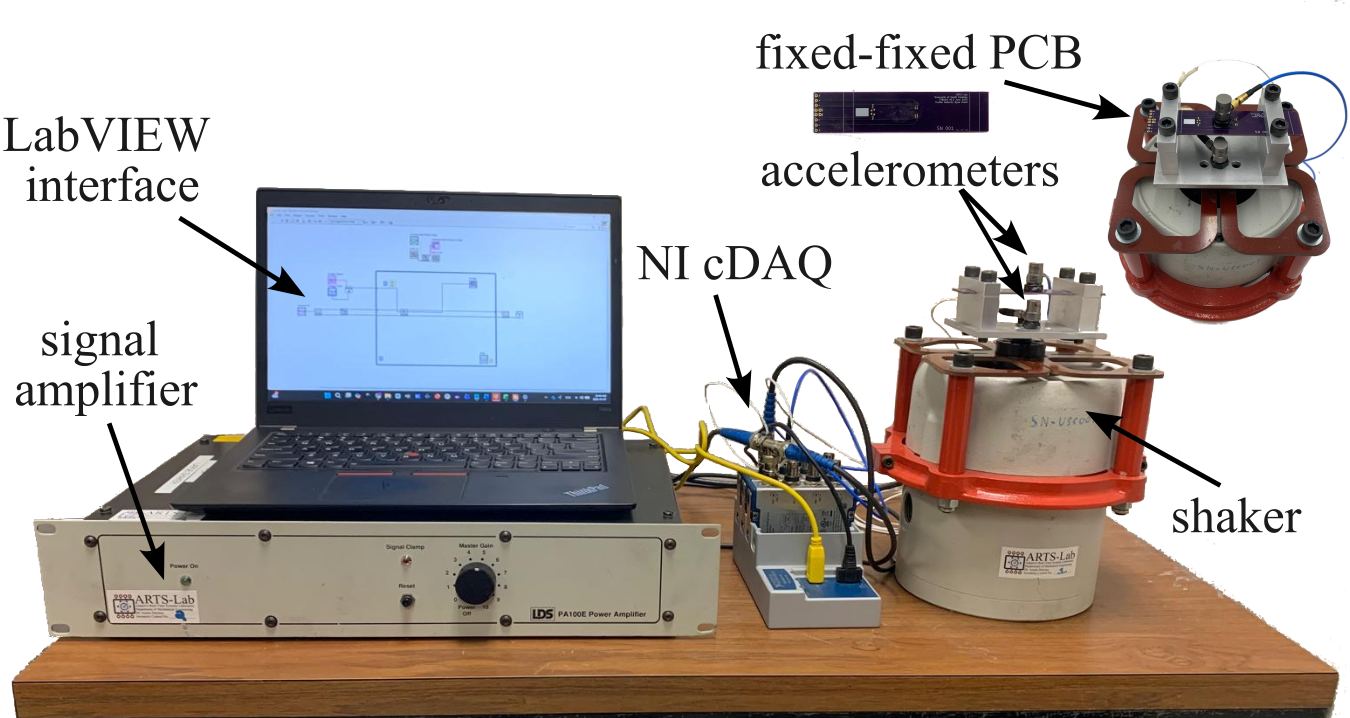
\includegraphics[width=\linewidth]{figures/data_acquisition.png}
	\caption{Experimental setup showing the fixed-fixed PCB assembly mounted on the shaker, together with the LabVIEW interface, signal amplifier, NI cDAQ, and accelerometers.}
	\label{fig:data_acquisition}
\end{figure}


The input excitation voltage applied to the shaker and the corresponding acceleration response measured on the PCB are shown in Figure~\ref{fig:excitation}(a). The input signal consists of a continuous low-amplitude harmonic excitation with a single impulsive shock superimposed at approximately 3.6~s. The output acceleration signal Figure~\ref{fig:excitation}(b), clearly captures the transient response induced by the shock. The acceleration trace clearly shows the steady-state harmonic vibration followed by a sharp transient spike at the instant the shock is applied, demonstrating the system’s dynamic reaction to the sudden impulse.


\begin{figure}[H]
	\centering
	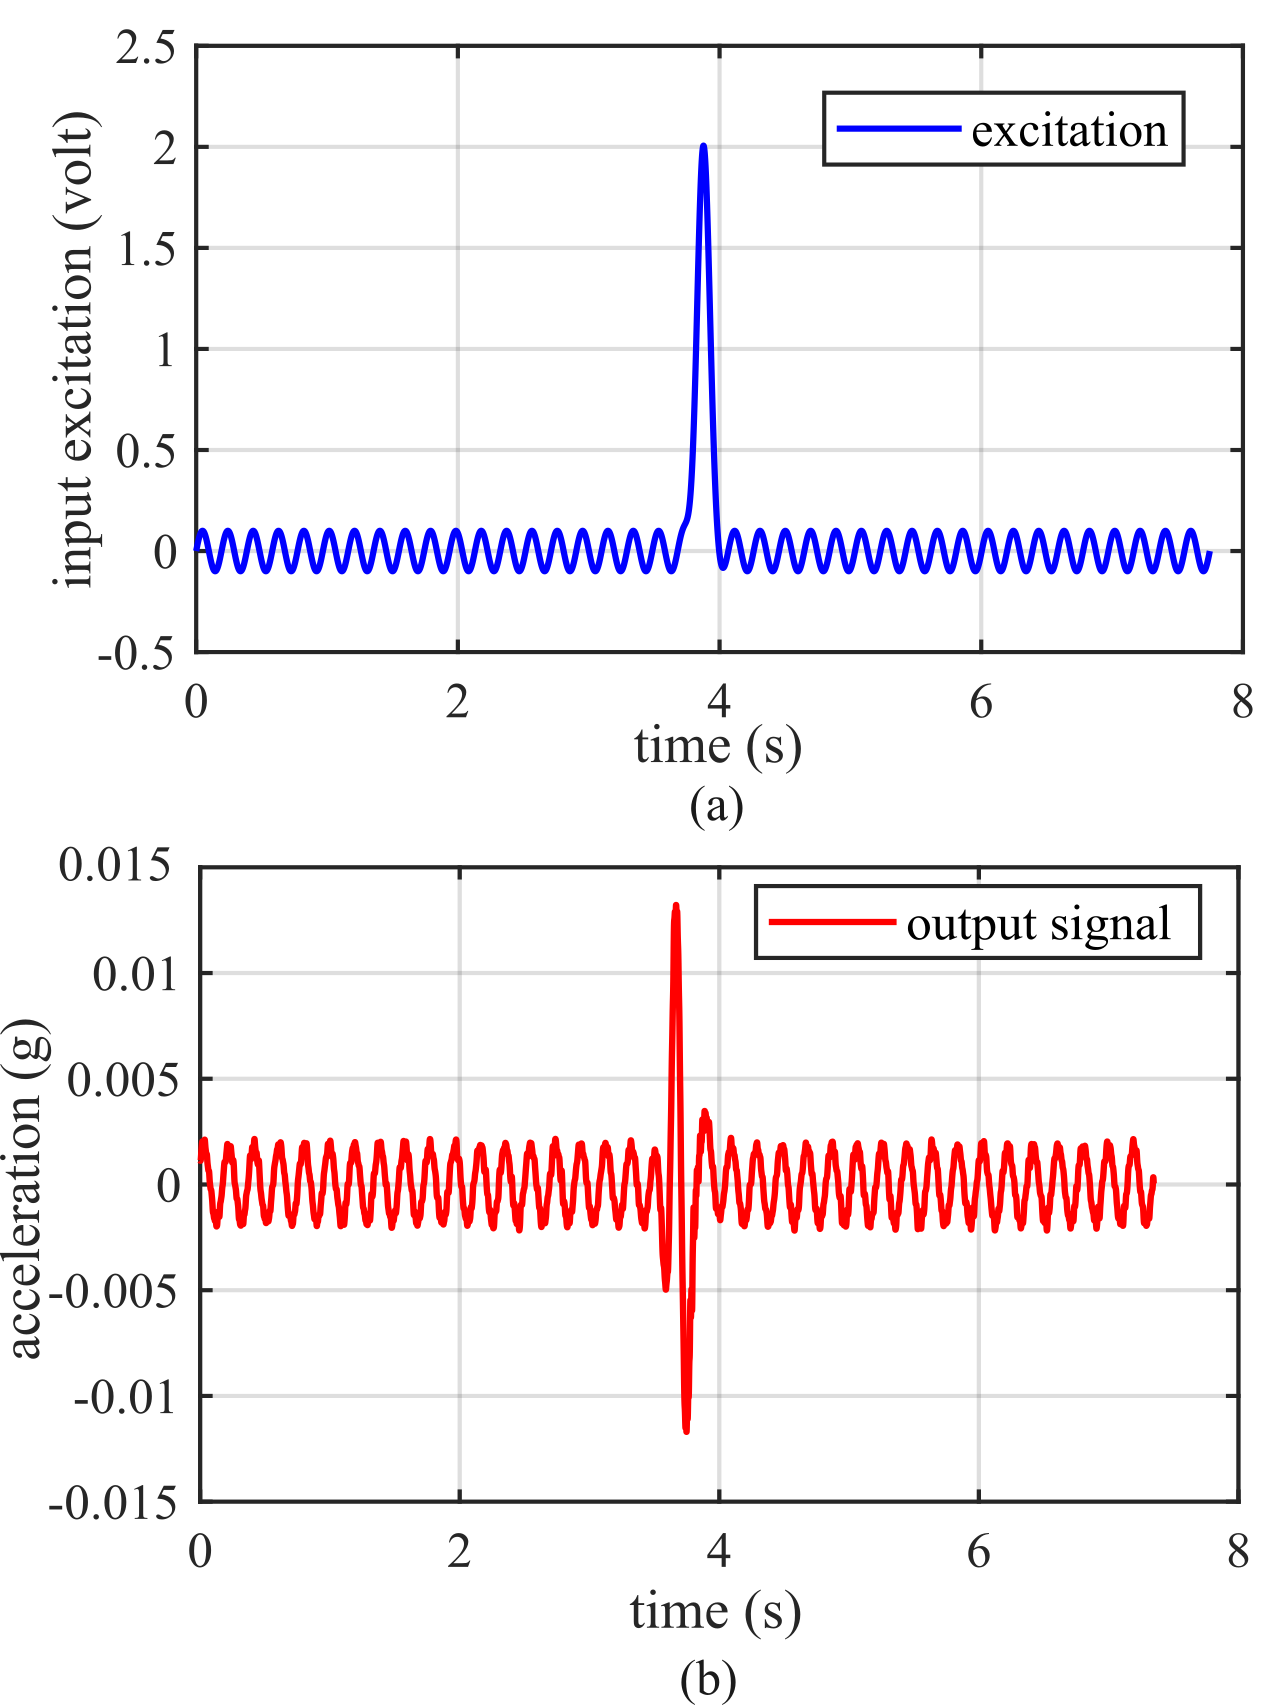
\includegraphics[width=\linewidth]{figures/input_output.png}
	\caption{Time histories of (a) input excitation voltage applied to the shaker and (b) output acceleration response measured on the fixed-fixed PCB.}
	\label{fig:excitation}
\end{figure}

These input-output signals constitute the raw high-rate time-series data used throughout this study. The sharp transient in the acceleration response at the shock instant produces a distinct change in the geometric pattern of the delay-embedded point cloud. This change is precisely what the proposed Fast TDA method detects in real time by monitoring the minor-axis length of the fitted ellipse, thereby enabling low-latency shock-onset identification.


%	\centering
%	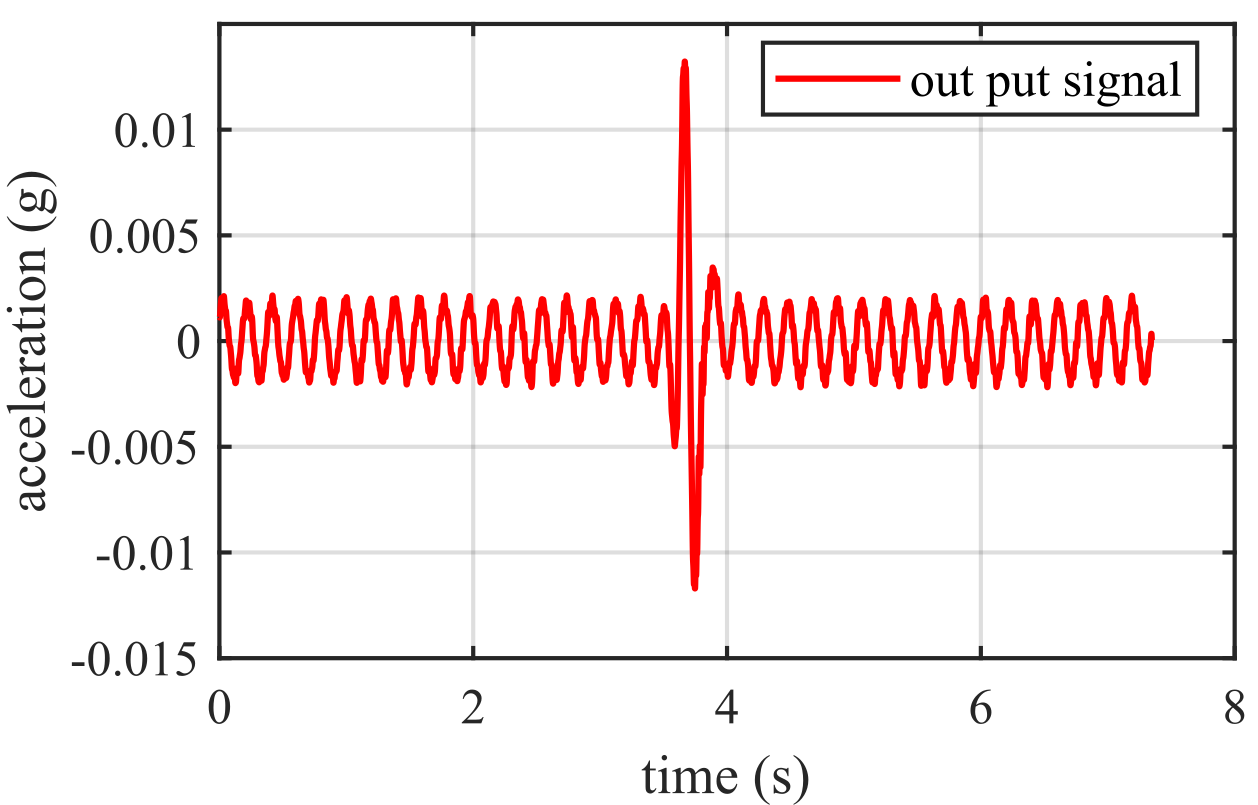
\includegraphics[width=\linewidth]{figures/output.png}
%	\caption{Output acceleration of PCB}
%	\label{fig:output}
%\end{figure}


 
%%%%%%%%%%%%% end figure %%%%%%%%%%%%%%%%%%%


%%%%%%%%%%%%%%%%%%%%%%%%%%%%%%%%%%%%%%%%%%%%%%%%%%%%%%%%%%%

%% Use title case for subsections and subsubsections (first letter of words capitalized)

\section{Mathematical derivation}

The general conic section is expressed as the algebraic implicit form:
\begin{equation}
	F(\mathbf{x};\,\mathbf{a}) \;=\;
	ax^2 + bxy + cy^2 + dx + ey + f \;=\; 0
	\label{eq:conic}
\end{equation}

where $\mathbf{x} = (x,,y)^\top$ is a 2D data point,
and $\mathbf{a} = [a,,b,,c,,d,,e,,f]^\top \in \mathbb{R}^6$
is the vector of conic parameters.
The parameters $[a,b,c]$ control the \emph{shape} of the conic,
while $[d,e,f]$ control its \emph{position} and \emph{scale}.
For the conic to represent an ellipse, the following conditions must be met:
discriminant condition must be satisfied:

\begin{equation}
	b^2 - 4ac \;<\; 0
	\label{eq:ellipse_cond}
\end{equation}

Given $N$ measured data points $\{(x_i,\,y_i)\}_{i=1}^{N}$,
the design matrix $\mathbf{D} \in \mathbb{R}^{N \times 6}$ is
constructed by expanding each point into the six conic basis terms:
$\mathbf{D}[i,:] = [x_i^2,\; x_iy_i,\; y_i^2,\; x_i,\; y_i,\; 1]$.
The $6\times6$ symmetric \emph{scatter matrix} is then:
\begin{equation}
	\mathbf{S} \;=\; \mathbf{D}^\top \mathbf{D}
	\label{eq:scatter}
\end{equation}
$\mathbf{S}$ is always $6\times6$ regardless of $N$,
making the downstream eigenvalue problem fixed in size
and directly suitable for FPGA hardware implementation.
The ellipse fitting problem seeks $\mathbf{a}$ that minimises
the sum of squared algebraic distances subject to the
ellipse-enforcing constraint $4ac - b^2 = 1$:
\begin{equation}
	\min_{\mathbf{a}} \;\;
	\mathbf{a}^\top \mathbf{S}\, \mathbf{a}
	\quad \text{subject to} \quad
	\mathbf{a}^\top \mathbf{C}\, \mathbf{a} \;=\; 1
	\label{eq:constrained}
\end{equation}

where $\mathbf{C} \in \mathbb{R}^{6\times6}$ is the constraint matrix
whose non-zero entries occupy only the upper-left $3\times3$ block
$\mathbf{C}_{11}$, reflecting that only $[a,b,c]$ are constrained:
\begin{equation}
	\mathbf{C}_{11} \;=\;
	\begin{bmatrix}
		0 & 0 & 2 \\
		0 & -1 & 0 \\
		2 & 0 & 0
	\end{bmatrix}
	\label{eq:C11}
\end{equation}

Applying Lagrange multipliers to \eqref{eq:constrained} yields
the \emph{generalised eigenvalue problem}:
\begin{equation}
	\mathbf{S}\,\mathbf{a} \;=\;
	\lambda\,\mathbf{C}\,\mathbf{a}
	\label{eq:gen_eig}
\end{equation}
where $\lambda$ is the Lagrange multiplier (eigenvalue) and
$\mathbf{a}$ is the corresponding eigenvector.
The optimal ellipse corresponds to the eigenvector
with the smallest positive eigenvalue $\lambda > 0$
that simultaneously satisfies condition~\eqref{eq:ellipse_cond}.
Since the lower-right $3\times3$ block of $\mathbf{C}$ is zero,
direct factorisation fails on the full $6\times6$ system.
Partitioning $\mathbf{S}$ into blocks according to
$[a,b,c]$ (rows/cols 1--3) and $[d,e,f]$ (rows/cols 4--6),
the unconstrained parameters $[d,e,f]$ are eliminated
analytically via the \emph{Schur complement}:
\begin{equation}
	\widetilde{\mathbf{S}} \;=\;
	\mathbf{S}_{11}
	\;-\;
	\mathbf{S}_{12}\,\mathbf{S}_{22}^{-1}\,\mathbf{S}_{21}
	\label{eq:schur}
\end{equation}
where $\mathbf{S}_{11}$ captures interactions among $[a,b,c]$,
$\mathbf{S}_{22}$ captures interactions among $[d,e,f]$,
and $\mathbf{S}_{12}=\mathbf{S}_{21}^\top$ captures cross-interactions.
$\widetilde{\mathbf{S}}$ is $3\times3$ and encodes the full
scatter information with the influence of $[d,e,f]$ already absorbed.
The constraint submatrix $\mathbf{C}_{11}$ is indefinite with
zero diagonal entries, requiring a permuted LDLT factorisation
with Bunch--Kaufman pivoting. A permutation $\mathbf{P}$
is determined such that:
\begin{equation}
	\mathbf{P}\,\mathbf{C}_{11}\,\mathbf{P}^\top
	\;=\; \mathbf{L}_3\,\mathbf{D}_3\,\mathbf{L}_3^\top
	\label{eq:ldlt}
\end{equation}
where $\mathbf{L}_3$ is $3\times3$ lower triangular with unit diagonal,
and $\mathbf{D}_3$ is block diagonal with non-zero determinant.
The subscript~3 denotes the $3\times3$ reduced system.
Using these factors, the reduced generalised eigenvalue problem is
transformed into the \emph{standard symmetric eigenvalue problem}:
\begin{equation}
	\mathbf{A}\,\mathbf{z} \;=\; \lambda\,\mathbf{z},
	\qquad
	\mathbf{A} \;=\;
	\mathbf{D}_3^{-1}\,\mathbf{L}_3^{-1}\,
	\widetilde{\mathbf{S}}_{\mathrm{p}}\,
	\mathbf{L}_3^{-\top}
	\label{eq:standard_eig}
\end{equation}
where $\widetilde{\mathbf{S}}_{\mathrm{p}} =
\mathbf{P}\,\widetilde{\mathbf{S}}\,\mathbf{P}^\top$
is the permuted Schur complement.
$\mathbf{A}$ is $3\times3$ and symmetric,
making it directly solvable by the cyclic Jacobi method on hardware.After solving \eqref{eq:standard_eig} via the cyclic Jacobi method,
the shape parameters are recovered from the selected eigenvector
$\mathbf{z}_k$ as:
$\mathbf{a}_1^* = \mathbf{L}_3^{-\top}\mathbf{z}_k$,
where $k$ is the index of the smallest positive eigenvalue
satisfying \eqref{eq:ellipse_cond}.
The position and scale parameters follow directly by matrix
multiplication with no further eigenvalue computation:
\begin{equation}
	\mathbf{a}^* \;=\;
	\begin{bmatrix}
		\mathbf{a}_1^* \\[4pt]
		\mathbf{a}_2^*
	\end{bmatrix}
	\;=\;
	\begin{bmatrix}
		\mathbf{L}_3^{-\top}\,\mathbf{z}_k \\[4pt]
		-\,\mathbf{S}_{22}^{-1}\,\mathbf{S}_{21}\,\mathbf{a}_1^*
	\end{bmatrix}
	\label{eq:final}
\end{equation}
where $\mathbf{a}_1^* = [a,b,c]^\top$ defines the ellipse shape
and $\mathbf{a}_2^* = [d,e,f]^\top$ defines its position and scale.

The ellipse fitting procedure is summarised in
Algorithm~\ref{alg:ellipse}.
The scatter matrix $\mathbf{S}$ is first assembled
from the $N$ data points, then reduced from $6\times6$
to $3\times3$ via the Schur complement, which eliminates
the unconstrained parameters $[d,e,f]$ analytically.
The LDLT factors $\mathbf{L}_3$, $\mathbf{D}_3$, and
permutation $\mathbf{P}$, pre-computed offline from the
fixed constraint matrix $\mathbf{C}_{11}$, are used to
form the standard symmetric matrix $\mathbf{A}$.
The cyclic Jacobi method then diagonalises $\mathbf{A}$,
and the valid ellipse solution is identified by testing
the eigenvalue sign and discriminant condition.
The shape parameters $[a,b,c]$ are recovered from the
selected eigenvector, and $[d,e,f]$ follow by a single
matrix multiplication.


\begin{algorithm}[h]
	\caption{Direct Ellipse Fitting Pipeline}
	\label{alg:ellipse}
	\begin{algorithmic}[1]
		\small
		\Require $N$ points $\{(x_i,y_i)\}_{i=1}^{N}$,\;
		threshold $\varepsilon$,\;
		offline constants $\mathbf{L}_3^{-1}$,
		$\mathbf{D}_3^{-1}$, $\mathbf{P}$
		\Ensure  $\mathbf{a}^* = [a,b,c,d,e,f]^\top$
		
		\Statex \textit{// Stage 1: build scatter matrix}
		\State $\mathbf{D}[i,:]\!\leftarrow\!
		[x_i^2,\,x_iy_i,\,y_i^2,\,x_i,\,y_i,\,1]$
		\hfill $\forall\, i$
		\State $\mathbf{S} \leftarrow \mathbf{D}^\top\mathbf{D}$
		\hfill \textit{always $6\times6$}
		
		\Statex \textit{// Stage 2: partition S and Schur complement}
		\State $\mathbf{S}_{11}\!\leftarrow\!\mathbf{S}(1{:}3,1{:}3)$,\;
		$\mathbf{S}_{12}\!\leftarrow\!\mathbf{S}(1{:}3,4{:}6)$,\;
		$\mathbf{S}_{22}\!\leftarrow\!\mathbf{S}(4{:}6,4{:}6)$
		\State $\widetilde{\mathbf{S}} \leftarrow
		\mathbf{S}_{11} -
		\mathbf{S}_{12}\mathbf{S}_{22}^{-1}\mathbf{S}_{21}$
		\hfill \textit{reduced to $3\times3$}
		
		\Statex \textit{// Stage 3: partition $\mathbf{C}_{11}$
			and form matrix $\mathbf{A}$}
		\State $\mathbf{P},\mathbf{L}_3,\mathbf{D}_3 \leftarrow
		\mathrm{ldl}(\mathbf{C}_{11})$
		\hfill \textit{offline, hardcoded on FPGA}
		\State $\mathbf{A} \leftarrow
		\mathbf{D}_3^{-1}\mathbf{L}_3^{-1}
		(\mathbf{P}\widetilde{\mathbf{S}}\mathbf{P}^\top)
		\mathbf{L}_3^{-\top}$
		\hfill \textit{symmetric, $3\times3$}
		
		\Statex \textit{// Stage 4: cyclic Jacobi solver}
		\State $\mathbf{Z} \leftarrow \mathbf{I}_3$
		\hfill \textit{initialise eigenvector matrix}
		\Repeat
		\State $(p,q)\leftarrow
		\arg\max_{p<q}|A_{pq}|$
		\hfill \textit{largest off-diagonal}
		\State $\tau \leftarrow
		(A_{qq}-A_{pp})/(2A_{pq})$
		\State $t \leftarrow
		\mathrm{sign}(\tau)/
		(|\tau|+\sqrt{1+\tau^2})$
		\State $c \leftarrow 1/\sqrt{1+t^2}$,\;
		$s \leftarrow tc$
		\hfill \textit{rotation in $(p,q)$ plane}
		\State $\mathbf{A}\leftarrow
		\mathbf{J}^\top\mathbf{A}\mathbf{J}$,\;
		$\mathbf{Z}\leftarrow\mathbf{Z}\mathbf{J}$
		\hfill \textit{rows/cols $p,q$ only}
		\Until{$\max_{p<q}|A_{pq}| < \varepsilon$}
		\hfill \textit{converged}
		
		\Statex \textit{// Stage 5: select valid ellipse eigenvector}
		\For{$k=1$ \textbf{to} $3$}
		\State $\mathbf{a}_1^{(k)}\leftarrow
		\mathbf{L}_3^{-\top}\mathbf{z}_k$
		\hfill \textit{$\mathbf{z}_k$ = column $k$ of $\mathbf{Z}$}
		\If{$\lambda_k>0$ \textbf{and}
			$b^2-4ac<0$}
		\State $\mathbf{a}_1^*\leftarrow
		\mathbf{a}_1^{(k)}$
		\hfill \textit{smallest valid $\lambda_k$}
		\EndIf
		\EndFor
		
		\Statex \textit{// Stage 6: recover $\mathbf{a}_1^*$
			and $\mathbf{a}_2^*$ separately}
		\State $\mathbf{a}_1^* = [a,b,c]^\top \leftarrow
		\mathbf{L}_3^{-\top}\,\mathbf{z}_{k^*}$
		\hfill \textit{ellipse shape}
		\State $\mathbf{a}_2^* = [d,e,f]^\top \leftarrow
		-\mathbf{S}_{22}^{-1}
		\mathbf{S}_{21}\,\mathbf{a}_1^*$
		\hfill \textit{position and scale}
		\State \Return
		$\mathbf{a}^*\!=\!
		[\mathbf{a}_1^{*\top},\,
		\mathbf{a}_2^{*\top}]^\top$
		\hfill \textit{complete $[a,b,c,d,e,f]^\top$}
		
	\end{algorithmic}
\end{algorithm}


The LDL$^T$ factors $\mathbf{L}_3^{-1}$, $\mathbf{D}_3^{-1}$, and $\mathbf{P}$ are computed once offline in MATLAB from the fixed constraint matrix $\mathbf{C}_{11}$ and hardcoded as constants in the Vitis HLS implementation, so no factorisation is required at runtime. The only iterative component is the Jacobi loop in Stage~4, which converges in a small number of sweeps for a $3\times3$ symmetric matrix and relies solely on fixed plane rotations and localised two-row/two-column updates, making it well suited for pipelined FPGA execution with deterministic latency.

The pipeline is deliberately designed to minimise runtime complexity on FPGA hardware. By performing the Schur complement reduction in Stage~2, the problem size is reduced from a full $6\times6$ system to a compact $3\times3$ symmetric eigenproblem, eliminating the three unconstrained parameters analytically and avoiding unnecessary computation. The offline pre-computation of the LDL$^T$ factors in Stage~3 further removes any matrix factorisation from the real-time path, leaving only matrix multiplications and the cyclic Jacobi iterations. Because the Jacobi solver operates exclusively with simple rotations and local updates, the entire algorithm executes with fixed, deterministic latency that is independent of the input data, which is essential for reliable high-rate shock detection.

\section{results and discussion}

The time evolution of the six ellipse parameters obtained from the Fast TDA pipeline is shown in Figure~\ref{fig:ellipse_parameters}(a). The parameters (a), (b), and (c) describe the quadratic form of the conic, namely, the shape and orientation of the ellipse, while (d), (e), and (f) control its position and scale. Prior to the shock event, which is approximately 3.5~s, all parameters remain nearly constant, reflecting the steady-state harmonic excitation of the system. At the instant of shock imposition, a sharp transient appears. Parameters (b) and (c) exhibit pronounced spikes, whereas (d), (e), and (a) show comparatively smaller deviations. These high spikes in the quadratic coefficients directly alter the shape of the orbit in the delay-embedded point cloud, demonstrating that the quadratic terms are highly responsive to sudden changes in the system dynamics.

To highlight sensitivity, the same coefficients are normalised using a min-max scaling procedure. For each parameter, the values are first shifted by their minimum and then divided by their range, with a safeguard that sets the range to unity when it falls below a small threshold to avoid division by zero. An additional vertical offset is applied to separate the traces for clear visualisation. The normalised traces shown in Figure~\ref{fig:ellipse_parameters}(b) reveal that parameter (a) produces the fastest excursions at the shock instant. This rapid response indicates that (a) is highly sensitive to the sudden deformation of the delay-embedded point cloud and can serve as a reliable monitoring feature. In comparison, parameters (b) and (c) also display noticeable variations, while the position parameter (e) shows alteration with delay rather than the other parameters. These results confirm that the quadratic coefficients, particularly (a), dominate the topological signature captured by Fast TDA.


\begin{figure}[h]
	\centering
	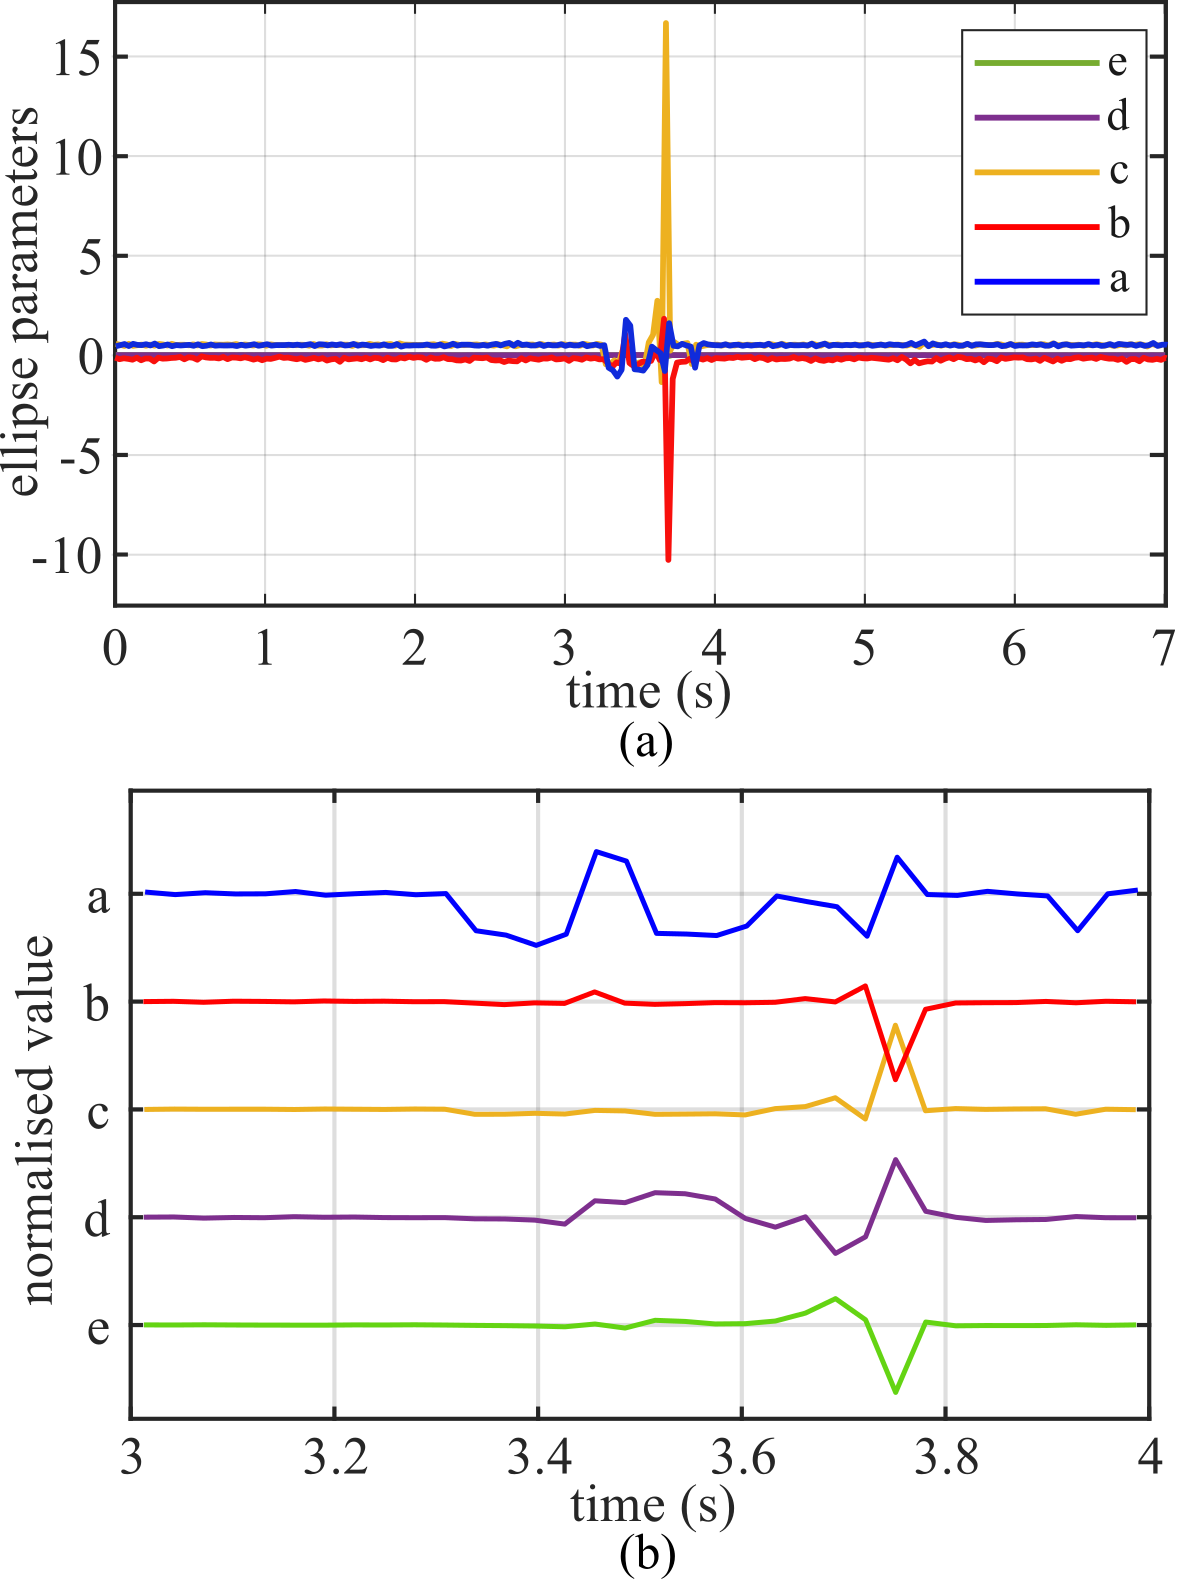
\includegraphics[width=\linewidth]{figures/ellipse_parameters.png}
	\caption{Time histories of the fitted ellipse parameters. (a) Raw coefficients (b) Normalised values of the same coefficients.}
	\label{fig:ellipse_parameters}
\end{figure}

\begin{figure*}[ht]
	\centering
	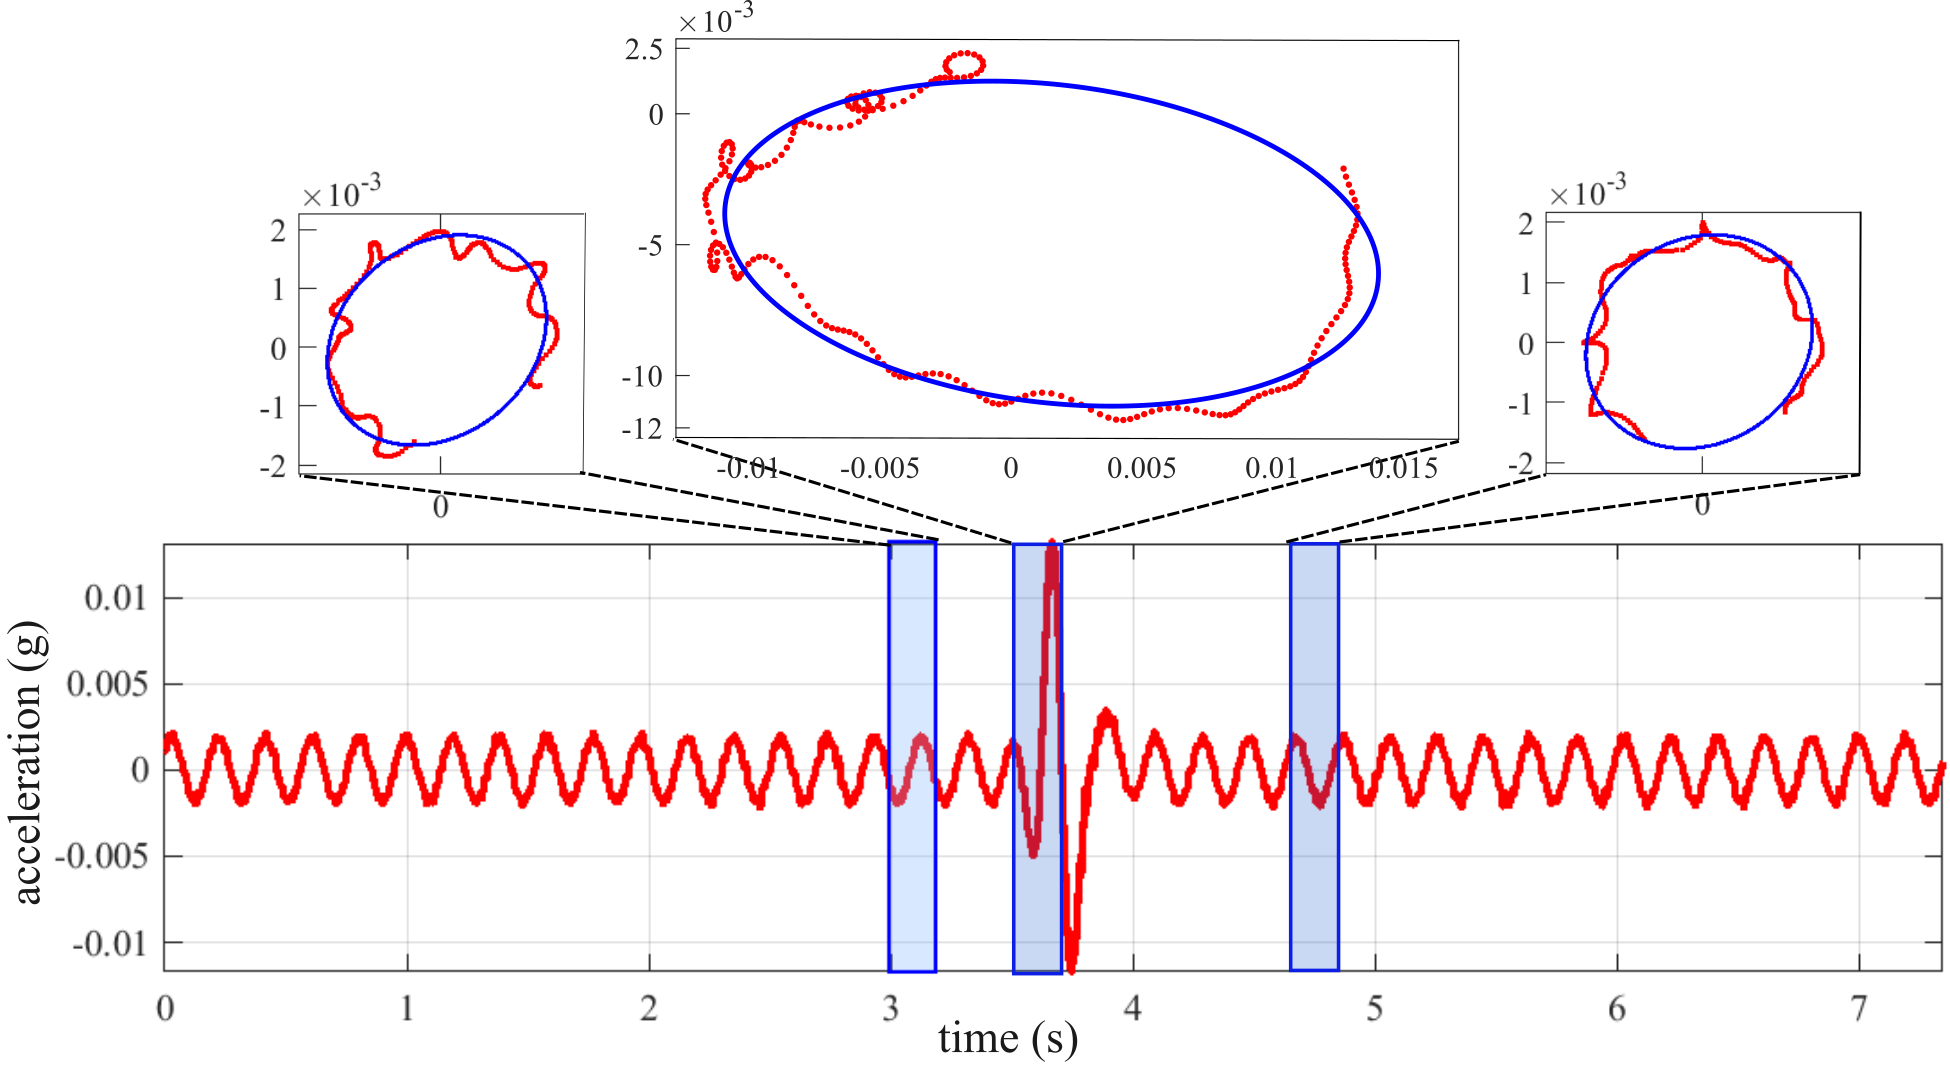
\includegraphics[width=\linewidth]{figures/signal_ellipse.png}
	\caption{Acceleration response with sliding windows indicating three representative intervals: pre-shock steady vibration, shock event, and post-shock which return to steady state. showing the display of the delay-embedded point cloud (blue) together with the fitted ellipse (red) at selected time instants.}
	\label{fig:signal_ellipse}
\end{figure*}

The corresponding evolution of the actual ellipse geometry is visualised in Figure~\ref{fig:signal_ellipse}. The main panel shows the acceleration time series with shaded windows marking three representative intervals as pre-shock with steady vibration, shock onset as a transient moment, and post-shock, returning to steady state. Inset ellipses superimposed on the delay-embedded point clouds illustrate the geometric change. Before the shock, the cloud forms a tight, nearly circular orbit; during the shock, the ellipse elongates dramatically and rotates; after the shock, the ellipse returns to a compact shape similar to the pre-shock condition. This visual evidence directly links the parameter transients observed in Figure~\ref{fig:ellipse_parameters} to measurable alterations in the point-cloud topology.

These three figures provide a consistent picture of how Fast TDA captures shock events. The raw and normalised parameter traces demonstrate that the quadratic coefficients, especially parameter (a), respond immediately and with large amplitude to the shock, while the geometric insets confirm that these coefficient changes translate directly into a pronounced deformation and rotation of the fitted ellipse. The ellipse returns to its original compact shape after the transient. This combination of rapid parameter fluctuation and visible orbit distortion supplies a clear and interpretable indicator of shock onset. The ability to detect such geometric changes without constructing persistence diagrams is the central advantage of the fast TDA approach and forms the foundation for low-latency real-time monitoring in high-rate systems.




\section{conclusion}


This study presented a real-time shock-onset detection framework for high-rate electronic and printed circuit board assemblies based on Fast TDA, an approximate topological approach that extracts geometric surrogates from delay-embedded point clouds. By replacing the computationally intensive construction of persistence diagrams with direct ellipse fitting on two-dimensional point clouds, the method achieves a dramatic reduction in processing time while retaining the essential topological signature of sudden transients. The ellipse-fitting stage was implemented as a fully hardware-optimised pipeline on an FPGA using a cyclic Jacobi solver for the underlying generalised eigenvalue problem, delivering deterministic low-latency operation suitable for high sampling rates. Experimental validation on a fixed-fixed beam platform subjected to controlled harmonic excitation followed by an imposed impulsive load demonstrated that the quadratic coefficients, particularly parameter \(a\), respond sharply to shock events and produce clear changes in the shape and orientation of the fitted ellipse. These geometric alterations were successfully captured by a sequential change-point detector, confirming that Fast TDA can localise shock onset with minimal delay and high robustness to steady-state vibration.

The proposed approach offers two primary advantages over conventional full TDA pipelines. First, it eliminates the need for persistence diagram computation at every time window, thereby enabling real-time execution on resource-constrained embedded hardware. Second, the ellipse parameters themselves serve as physically interpretable monitoring features that directly reflect changes in the underlying system dynamics. The framework, therefore, provides both low-latency detection performance and a transparent geometric interpretation of the detected events. These attributes make Fast TDA particularly well-suited for safety-critical applications in high-rate environments where rapid and reliable shock identification is essential.

Future work will focus on the complete hardware implementation of the Fast TDA algorithm on an FPGA using High-Level Synthesis (HLS). With the promising results already obtained from the current FPGA-accelerated ellipse fitting pipeline. This development will include integration of the change-point detection logic on the same FPGA, further optimisation for higher sampling rates, and extensive experimental validation on additional high-rate platforms. Overall, the results demonstrate that approximate topological analysis combined with efficient FPGA implementation constitutes a promising pathway toward practical, real-time structural health monitoring in high-rate dynamic systems.







%%%%% Acknowledgments %%%%%%%%%%%%%%%%%%%%%%%%%%%

\section*{Acknowledgments}
Place any acknowledgments here.


%%%  REFERENCES  %%%%%%%%%%%%%%%%%%%%%%%%%%%%%%%%
%%
%% Put your references into your .bib file in the usual way. Run latex once, bibtex once, then latex twice.
%% The asmeconf.bst style allows @inproceedings and @proceedings to include: 
%%		venue = {Location of Conference}, 
%%		eventdate = {Month, days},

\nocite{*}%% <=== Delete this line unless you want to typeset the entire contents of your .bib file !!

\bibliographystyle{asmeconf}  %% .bst file following ASME conference format. Do not change.
\bibliography{references}%% <=== change this to the name of your bib file




%%%%%%%%%%%%%%%%%%%%%%%%%%%%%%%%%%%%%%%%%%%%%%%%%%%%%%%%%%%%%%%%%%%%%%%%%%%%%%%%%%%%%%

\end{document}

